\chapter{Another test chapter}

\begin{algorithm}
	\small
	\begin{shaded}
		\begin{algorithmic}[1]
			\newcommand*{\To}{\textbf{to}\xspace}
			\newcommand*{\Init}{\State\textbf{init}\xspace}
			\newcommand*{\B}{\mathcal{B}}
			\Init \(M \gets 0 \in \B^{N \times r}\) \Comment{Result matrix}
			\For{ \(i \gets 1\) \To N}
				\For{ \(j \gets r - r_1 + 1\) \To \(r\)}
					\State \(\ell \gets \) \Call{RandomSelect}{$\{1, \ldots, j - 1\}$} \Comment{Uniformly select set entry}
					\If{\({M}[i,\ell] = 1\)}
						\State \({M}[i,j] \gets 1\)
					\Else
						\State \({M}[i,\ell] \gets 1\)
					\EndIf
				\EndFor
			\EndFor
		\end{algorithmic}
	\end{shaded}
	\caption[Uncorrelated random data generation]{Algorithm for the generation of a block $M$ of $N$ uncorrelated random vectors of length $r$, containing exactly $r_1$ ones.}
	\label{alg:binam_random_data}
\end{algorithm}

\epigraph{To test is to live. To believe is to die.}{Anonymous Heretic}
\marginnote{Yes, this is just a test. If you read this, you are most likely doomed.}
\blindtext

\begin{figure}
    \centering
    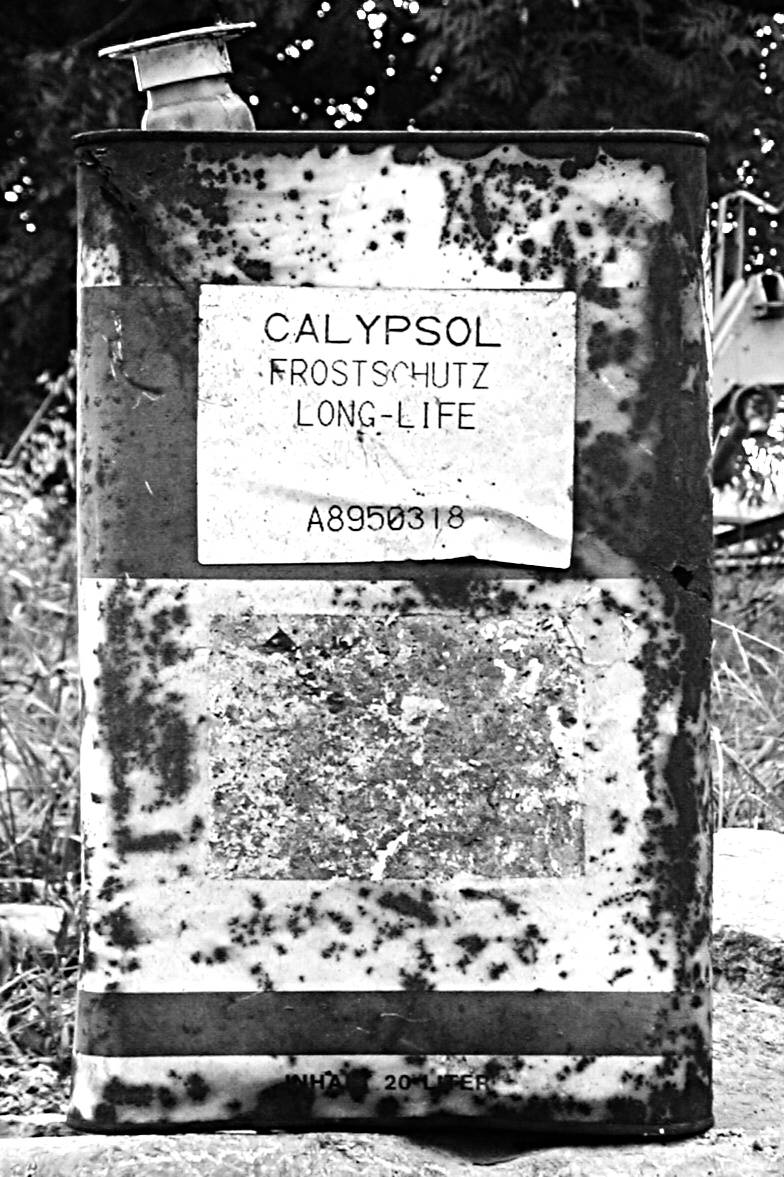
\includegraphics[width=8cm]{demo.png}
    \caption{Truly a fine canister, comparable only to mjollnir.}
    \label{fig:canister}
\end{figure}

\Blindtext\Blindtext

A picture says more than a thousand words (see \cref{fig:canister}).

\section{The Throat of the World}

\marginnote{Margin notes help to add structure to long runs of text}
\blindtext

\blindlistlist[2]{itemize}

\section{The Silence Has Been Broken}

\marginnote{Test test test}\blindtext

\blindlistlist[2]{enumerate}

\section{Discerning the Transmundane}

\marginnote{You can even add small formulas, like this one:
\begin{align*}
\sum_{i=1}^{n} i &= n \cdot \frac{n + 1}2
\end{align*}}
\blindtext

\subsection{Composure, Speed, and Precision}

\marginnote{Or this one:
\begin{align*}
E &= mc^2
\end{align*}}
\blindtext

\section{Implementation}

\blindtext

\begin{lstlisting}[caption={Very sophisticated code example.},label=lst:example]
function fizzbuzz(upperBound) {
    for (let i = 1; i < upperBound; i++) {
        if (i % 15 == 0) {
            console.log("FizzBuzz");
        } else if (i % 3 == 0) {
            console.log("Fizz");
        } else if (i % 5 == 0) {
            console.log("Buzz");
        } else {
            console.log(i);
        }
    }
}
\end{lstlisting}
